\section{Studio gas ignoto}
Sostituendo la sorgente nota con una incognita, ci è stato possibile sfruttare la legge di Cauchy appena verificata per risalire al valore delle lunghezze d’onda che abbiamo osservato.
La procedura sperimentale è identica e consiste nella stima degli indici di rifrazione associati alle righe di emissione più intense della sorgente incognita.
\subsection{Prima sorgente ignota}
La seguente tabella riassume le misure raccolte
\begin{table}[h!]
    \centering
    \begin{tabular}{ccc}
    \toprule
    $n$ && $\lambda\,(\angstrom)$ $(10^{-5})$ \\
    \midrule
    1,66423  &&  95\\
    1,64990  &&  96\\
    1,64197  &&  98\\
    1,63546  &&  99\\
    1,63463  &&  996\\
    1,63295  &&  100\\
    1,63211  &&  100\\
    1,62992  &&  101\\
    1,62992  &&  101\\
    \bottomrule
    \end{tabular}
    \caption{}
    \label{tab:my_label}
\end{table}

A questo punto invertendo la legge di Cauchy è possibile risalire a $\lambda$ e la sua incertezza
\begin{equation}
\lambda= \sqrt{\dfrac{B}{n-A}}
\label{lambda}
\end{equation}
\begin{equation}
\sigma_\lambda^2=\frac{1}{4(n-A)^{2}}\left(\lambda^{2}\left(\sigma_{A}^{2}+\sigma_{n}^{2}\right)+2 \sigma_{A B}^{2}+\frac{\sigma_{B}^{2}}{\lambda^{2}}\right)
\label{sigma lambda}
\end{equation}
I risultati del fit sono riportati nella Figura \ref{confronto 1}.
\begin{figure}[h!]
    \centering
    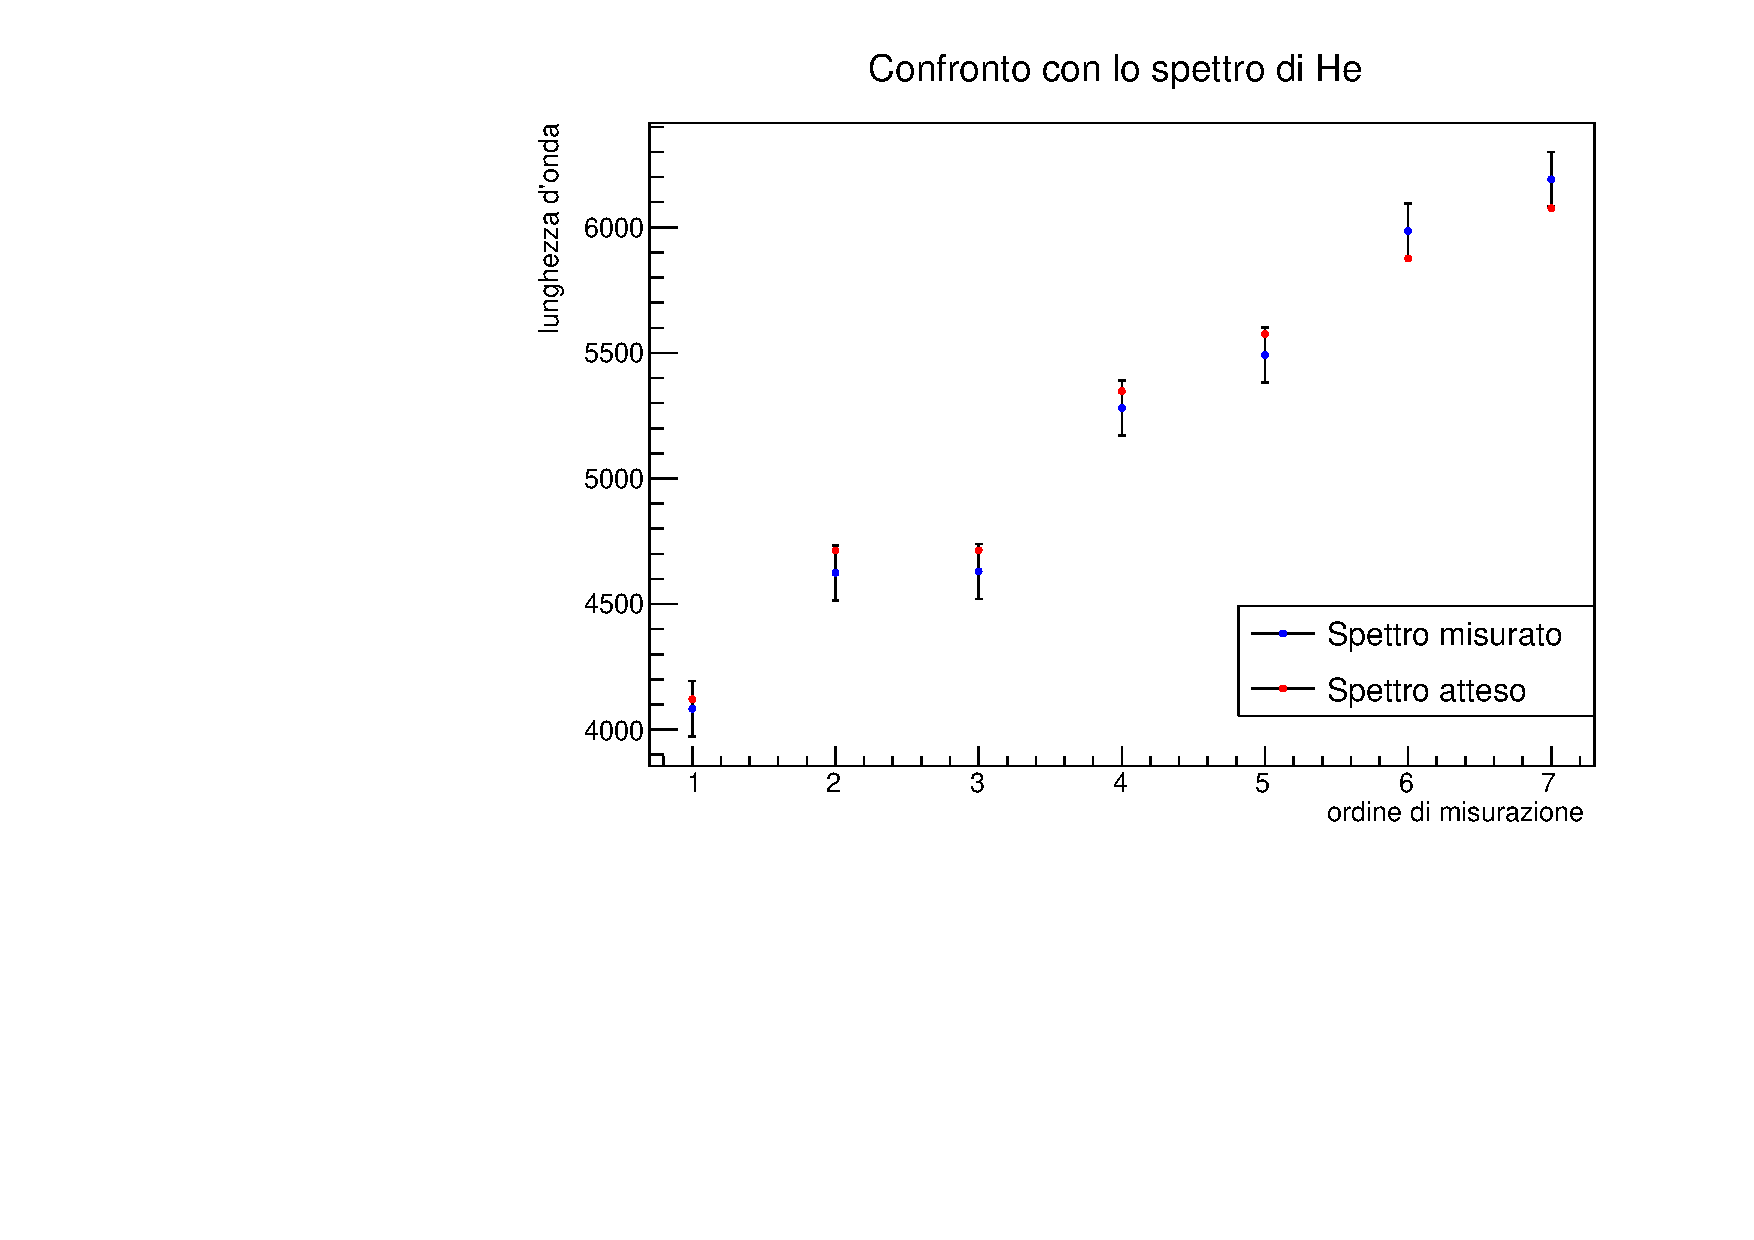
\includegraphics[scale=.6]{Immagini/Confronto 1.pdf}
    \caption{}
    \label{confronto 1}
\end{figure}
\subsection{Seconda sorgente ignota}
La tabella \ref{tabella 8} riassume le misure raccolte. Successivamente tramite le Eq. \ref{lambda} e \ref{sigma lambda} si ricavano i valori di $\lambda$ e $\sigma^2_\lambda$. I risultati del confronto sono riportati nella Figura  \ref{confronto 2}.
\begin{table}[h!]
    \centering
    \begin{tabular}{cc}
    \toprule
    $n$ & $\lambda$ ($\angstrom$)\\
    \midrule
    1,6350	&5946,74\\
    1,6370	&5730,32\\
    1,6450	&5056,89\\
    1,6587	&4301,91\\
    1,6613	&4194,11\\
    1,6662	&4012,93\\
    1,6734	&3782,16\\
    \bottomrule
    \end{tabular}
    \caption{}
    \label{tabella 8}
\end{table}
\begin{figure}[h!]
    \centering
    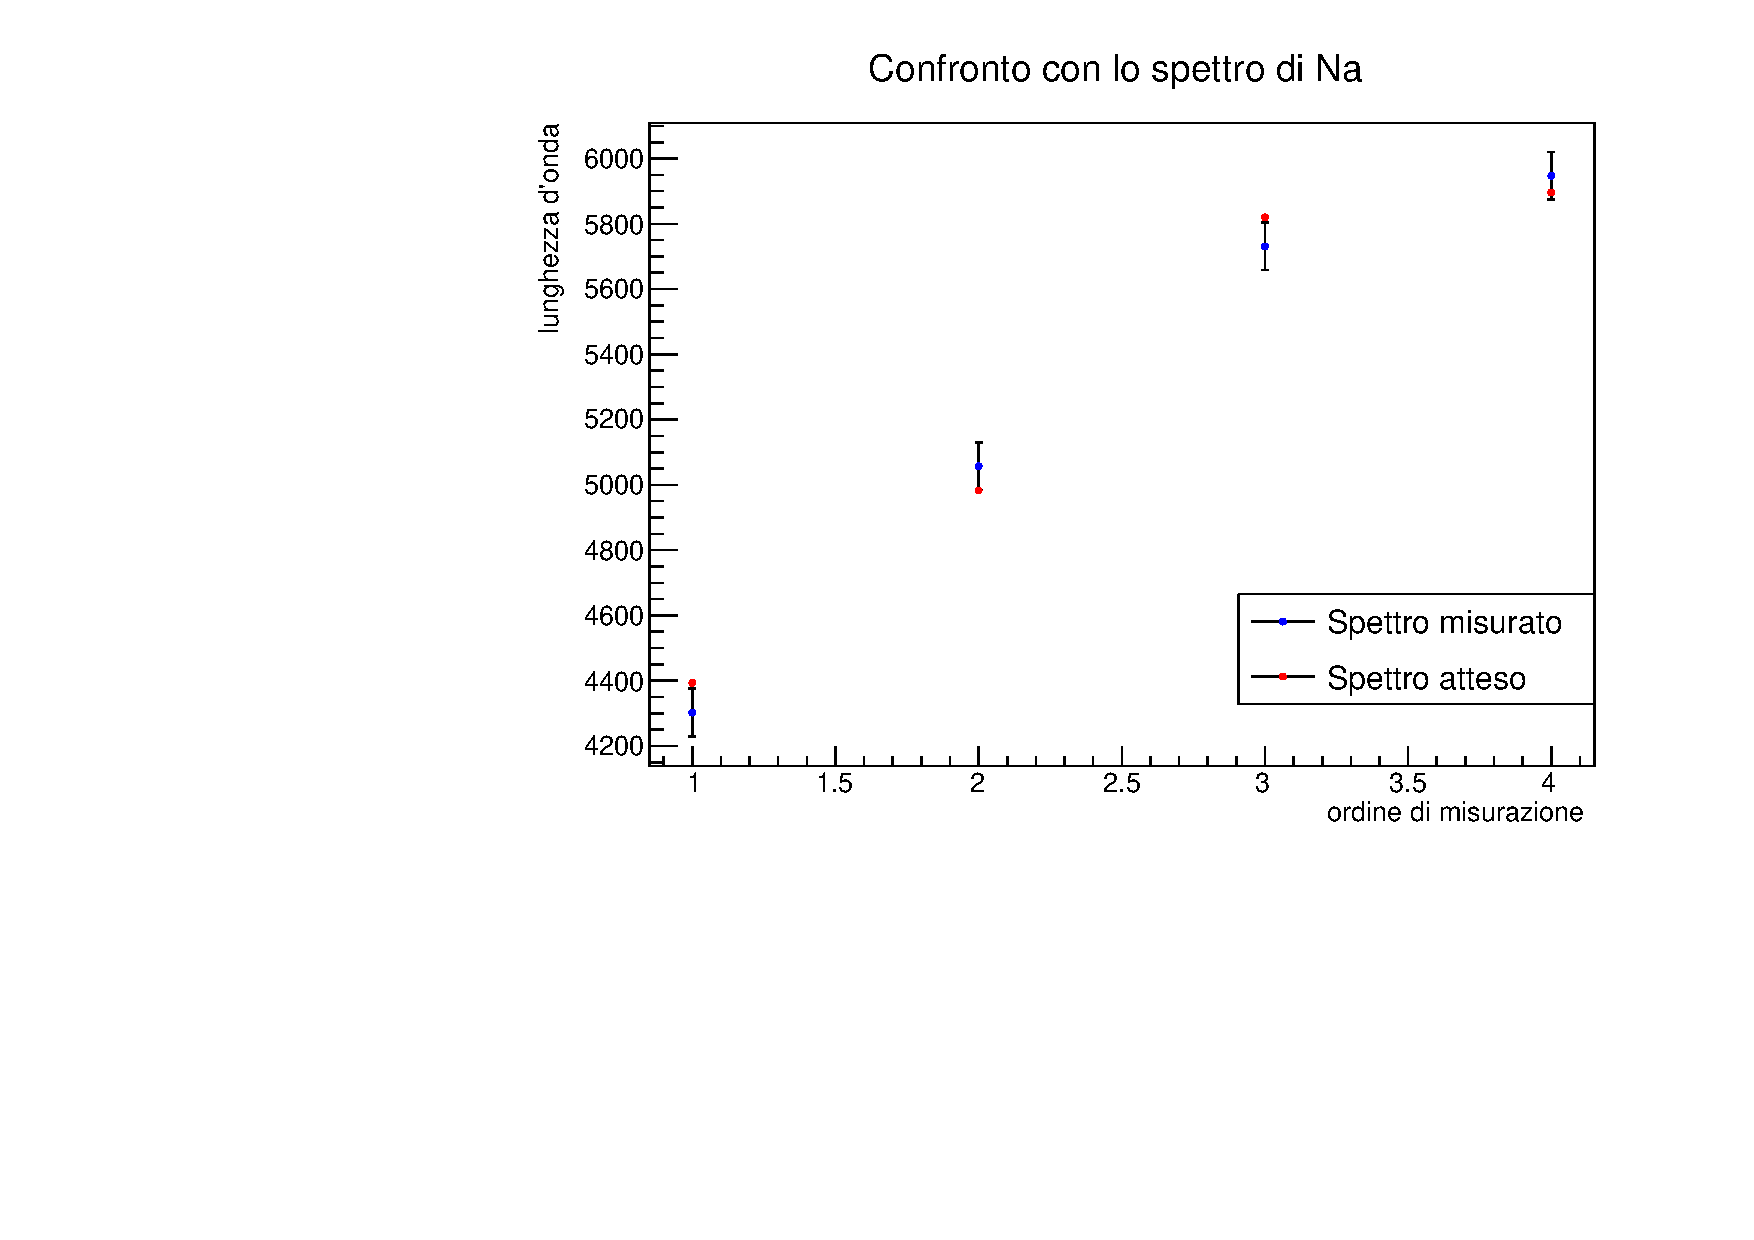
\includegraphics[scale=.6]{Immagini/Confronto 2.pdf}
    \caption{}
    \label{confronto 2}
\end{figure}
\subsection{Considerazioni sui gas determinati}
Confrontando i valori ottenuti con quelli tabulati per i gas nobili, si osserva una forte compatibilità con le righe di emissione dell’Elio e del Sodio, seppur con un certo bias. Si nota infatti che non è presente una regolarità nell'andamento della posizione della $\lambda$ misurata, se sopra se sotto, rispetto a ciò che ci si attende. Il seguente grafico mostra qualitativamente tale bias.

La natura di questo bias non è pienamente chiara: potrebbe trattarsi di una stima errata di $\vartheta_0$ o di $\alpha$, presente, quindi, fin dall’inizio dell’esperienza. Dato che abbiamo cercato di effettuare le misure nel modo più preciso possibile, un’ipotesi che è possibile avanzare riguarda la struttura geometrica del prisma: infatti, la presenza di vertici smussati potrebbe aver fatto sì che la luce non incidesse su uno spigolo perfettamente verticale ma su una superficie lievemente irregolare.
Questa ipotesi può trovare conferma nella forma righe di emissione che, viste dal telescopio, sono risultate essere incurvate e non perfettamente verticali. Ciò nonostante, dare una stima quantitativa di questa perturbazione risulta essere difficoltoso e quindi la misura viene giudicata allo stesso modo accettabile.
